%%%%%%%%%%%%%%%%%%%%%%%%%%%%%%%%%%%%%%%%%%%%%%%
%%%     Declarations (skip to Begin Document, line 88, for parts you fill in)
%%%%%%%%%%%%%%%%%%%%%%%%%%%%%%%%%%%%%%%%%%%%%%%

\documentclass[10pt]{article}

\usepackage{geometry}  % Lots of layout options.  See http://en.wikibooks.org/wiki/LaTeX/Page_Layout
\geometry{letterpaper}  % ... or a4paper or a5paper or ... 
\usepackage{fullpage}  % somewhat standardized smaller margins (around an inch)
\usepackage{setspace}  % control line spacing in latex documents
\usepackage[parfill]{parskip}  % Activate to begin paragraphs with an empty line rather than an indent

\usepackage{amsmath,amssymb}  % latex math
\usepackage{empheq} % http://www.ctan.org/pkg/empheq
\usepackage{bm,upgreek}  % allows you to write bold greek letters (upper & lower case)

\usepackage{soul}  % for hl and friends

% for typsetting algorithm pseudocode see http://en.wikibooks.org/wiki/LaTeX/Algorithms_and_Pseudocode
\usepackage{algorithmic,algorithm}  

\usepackage{graphicx}  % inclusion of graphics; see: http://en.wikibooks.org/wiki/LaTeX/Importing_Graphics
% allow easy inclusion of .tif, .png graphics
\DeclareGraphicsRule{.tif}{png}{.png}{`convert #1 `dirname #1`/`basename #1 .tif`.png}

\usepackage{subfigure}  % allows subfigures in figure

\usepackage{xspace}
\newcommand{\latex}{\LaTeX\xspace}

\usepackage{color}  % http://en.wikibooks.org/wiki/LaTeX/Colors

\long\def\ans#1{{\color{blue}{\em #1}}}
\long\def\ansnem#1{{\color{blue}#1}}
\long\def\boldred#1{{\color{red}{\bf #1}}}
\long\def\boldred#1{\textcolor{red}{\bf #1}}
\long\def\boldblue#1{\textcolor{blue}{\bf #1}}

% Useful package for syntax highlighting of specific code (such as python) -- see below
\usepackage{listings}  % http://en.wikibooks.org/wiki/LaTeX/Packages/Listings
\usepackage{textcomp}

%%% The following lines set up using the listings package
\renewcommand{\lstlistlistingname}{Code Listings}
\renewcommand{\lstlistingname}{Code Listing}

%%% Specific for python listings
\definecolor{gray}{gray}{0.5}
\definecolor{green}{rgb}{0,0.5,0}

\lstnewenvironment{python}[1][]{
\lstset{
language=python,
basicstyle=\footnotesize,  % could also use this -- a little larger \ttfamily\small\setstretch{1},
stringstyle=\color{red},
showstringspaces=false,
alsoletter={1234567890},
otherkeywords={\ , \}, \{},
keywordstyle=\color{blue},
emph={access,and,break,class,continue,def,del,elif ,else,%
except,exec,finally,for,from,global,if,import,in,i s,%
lambda,not,or,pass,print,raise,return,try,while},
emphstyle=\color{black}\bfseries,
emph={[2]True, False, None, self},
emphstyle=[2]\color{green},
emph={[3]from, import, as},
emphstyle=[3]\color{blue},
upquote=true,
morecomment=[s]{"""}{"""},
commentstyle=\color{gray}\slshape,
emph={[4]1, 2, 3, 4, 5, 6, 7, 8, 9, 0},
emphstyle=[4]\color{blue},
literate=*{:}{{\textcolor{blue}:}}{1}%
{=}{{\textcolor{blue}=}}{1}%
{-}{{\textcolor{blue}-}}{1}%
{+}{{\textcolor{blue}+}}{1}%
{*}{{\textcolor{blue}*}}{1}%
{!}{{\textcolor{blue}!}}{1}%
{(}{{\textcolor{blue}(}}{1}%
{)}{{\textcolor{blue})}}{1}%
{[}{{\textcolor{blue}[}}{1}%
{]}{{\textcolor{blue}]}}{1}%
{<}{{\textcolor{blue}<}}{1}%
{>}{{\textcolor{blue}>}}{1},%
%framexleftmargin=1mm, framextopmargin=1mm, frame=shadowbox, rulesepcolor=\color{blue},#1
framexleftmargin=1mm, framextopmargin=1mm, frame=single,#1
}}{}
%%% End python code listing definitions

\DeclareMathOperator{\diag}{\texttt diag}
\DeclareMathOperator{\cov}{\texttt cov}

%%%%%%%%%%%%%%%%%%%%%%%%%%%%%%%%%%%%%%%%%%%%%%%
%%%     Begin Document
%%%%%%%%%%%%%%%%%%%%%%%%%%%%%%%%%%%%%%%%%%%%%%%

\begin{document}

\begin{center}
    {\Large {\bf ISTA 421/521 -- Homework 3}} \\
    \boldred{Due: Friday, October 5, 5pm} \\
    20 pts total for Undergrads, 25 pts total for Grads
    
\end{center}

\begin{flushright}
Ken Youens-Clark

Graduate 
\end{flushright}

N.B.: I consulted with graduate students Kai Blumberg and Matthew Miller.

\vspace{1cm}


%%%%%%%%%%%%%%%%
%%%     Problems
%%%%%%%%%%%%%%%%

\begin{itemize}

%%%     Problem 1
\item[1.] [2 points]
Adapted from {\bf Exercise 2.3} of FCML:

Let $Y$ be a random variable that can take any non-negative integer value.  The likelihood of these outcomes is given by the Poisson pmf (probability mass function):
\begin{eqnarray}
p(y) = {\lambda^y\over y!} e^{-\lambda}
\end{eqnarray}
By using the fact that for a discrete random variable the pmf gives the probabilities of the individual events occurring and the probabilities are additive...
\begin{enumerate}
\item[(a)] Compute the probability that $Y \geq 5$ and $Y \leq 10$ for $\lambda = 7$, i.e., $P(5 \leq Y \leq 10)$.  Write a (very!)~short python script to compute this value, and include a listing of the code in your solution.
\item[(b)] Using the result of (a) and the fact that one outcome has to happen, compute the probability that $Y < 5$ or $Y > 10$.
\end{enumerate}

{\bf Solution.} %$<$Solution goes here$>$

\begin{verbatim}
#!/usr/bin/env python3
#
# INFO521 Homework 3 Problem #1 (Poisson pmf)
# Author: Ken Youens-Clark
# Sept 29, 2018
#

import numpy as np

lam = 7
tot = 0
for y in range(5,11):
    r = (np.power(lam, y) / np.math.factorial(y)) * np.exp(-1 * lam)
    print('y({:2}, {}) = {:.02f}'.format(y, lam, r))
    tot += r

print('--------   ----'.format(tot))
print('total    = {:.02f}'.format(tot))

$ ./poisson.py
y( 5, 7) = 0.13
y( 6, 7) = 0.15
y( 7, 7) = 0.15
y( 8, 7) = 0.13
y( 9, 7) = 0.10
y(10, 7) = 0.07
--------   ----
total    = 0.73
\end{verbatim}

$P(5 \leq Y \leq 10) = 0.73$, therefore $P(Y < 5$ or $Y > 10) = (1 - 0.73) = 0.27$

%%%     Problem 2
\item[2.] [3 points]
Adapted from {\bf Exercise 2.4} of FCML:

Let $X$ be a random variable with uniform density, $p(x) = \mathcal{U}(a,b)$.  \\
Work out analytically $\mathbf{E}_{p(x)} \left\{ 35 + 3x - 0.5x^3 + 0.05x^4 \right\}$ for $a=-4$, $b=10$ (show the steps).  

The script {\tt approx\_expected\_value.py} demonstrates how you use random samples to approximate an expectation, as described in Section 2.5.1 of FCML.  The script estimates the expectation of the function $y^2$ when $Y \sim \mathcal{U}(0,1)$ (that is, $Y$ is uniformly distributed between $0$ and $1$).  This script shows a plot of how the estimation improves as larger samples are considered, up to 1000 samples.

Modify the script {\tt approx\_expected\_value.py} to compute a sample-based approximation to the expectation of the function $35 + 3x - 0.5x^3 + 0.05x^4$ when $X \sim \mathcal{U}(-4,10)$ and observe how the approximation improves with the number of samples drawn.  Include a plot showing the evolution of the approximation, relative to the true value, over 5,000 samples.

{\bf Solution.}

\begin{eqnarray*}
\begin{aligned}
p(x) &= \mathcal{U}(a,b) = \frac{1}{b-a} = \frac{1}{10 - (-4)} = \frac{1}{14}
\\
\mathbf{E}_{p(x)} \left\{ 35 + 3x - 0.5x^3 + 0.05x^4 \right\} 
&= \int_{x=-4}^{10} 35 + 3x - 0.5x^3 + 0.05x^4 p(x) dx
\\
&= \int_{x=-4}^{10} \frac{35 + 3x - 0.5x^3 + 0.05x^4}{14} dx
\\
&= \left[ \frac{35x + \frac{3}{2}x^2 - \frac{0.5}{4}x^4 + \frac{0.05}{5}x^5}{14} \right]_{-4}^{10}
\\
&= \frac{((35 * 10) + (1.5 * 100) - (0.125 * 10000) + (0.01 * 100000))}{14}
\\
& - \frac{((35 * -4) + (1.5 * 16)  - (0.125 * 256 ) + (0.01 * -1024) )}{14}
\\
&= \frac{(350 + 150 - 1250 + 1000)}{14} - \frac{(-140 + 24 - 32 - 10.24)}{14}
\\
&= \frac{250 + 158.24}{14}
\\
&= \frac{408.24}{14}
\\
&= 29.16
\end{aligned}
\end{eqnarray*}

\begin{figure}[H]
\centering
  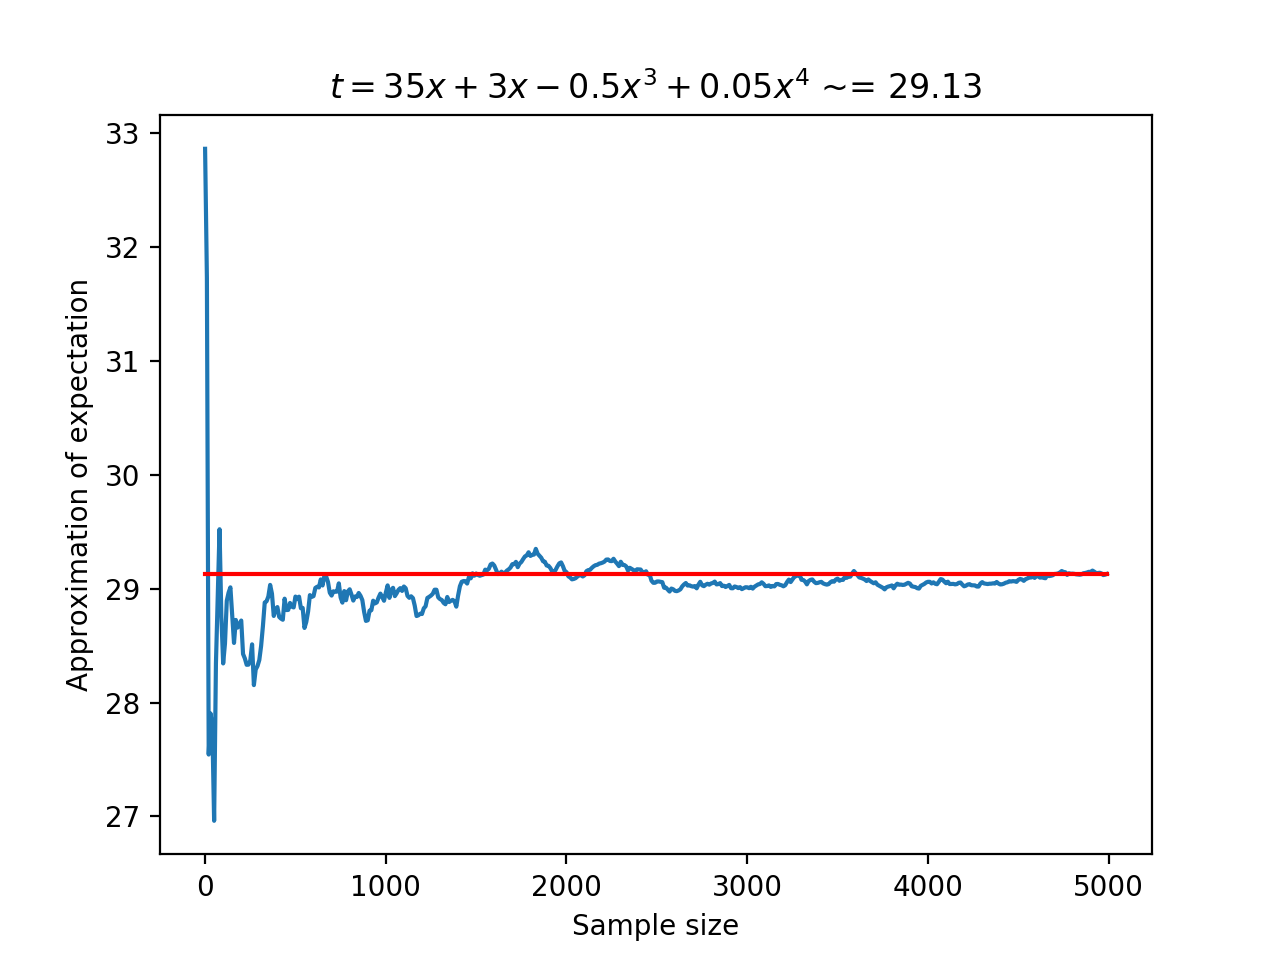
\includegraphics[width=\linewidth]{approx.png}
 \caption{Sample-based approximation}
\label{label}
\end{figure}

%%%     Problem 3
\item[3.] [2 points; \boldred{Required only for Graduates}]
Adapted from {\bf Exercise 2.6} of FCMA:

Assume that $p(\mathbf{w})$ is the Gaussian pdf for a $D$-dimensional vector $\mathbf{w}$ given in
\begin{eqnarray}
p(\mathbf{w}) = \frac{1}{(2 \pi)^{D/2} | \mathbf{\Sigma} |^{1/2}} \exp \left\{ -\frac{1}{2} (\mathbf{w} - \boldsymbol{\mu})^\top \mathbf{\Sigma}^{-1} (\mathbf{w} - \boldsymbol{\mu}) \right\} . \label{eqn:multnormal}
\end{eqnarray}

Suppose we use a diagonal covariance matrix with different elements on the diagonal, i.e.,
\begin{eqnarray*}
\mathbf{\Sigma} = 
\begin{bmatrix}
\sigma_1^2 & 0 & \cdots & 0 \\
0 & \sigma_2^2 & \cdots & 0 \\
\vdots & \vdots & \ddots & \vdots \\
0 & 0 & \cdots & \sigma_D^2
\end{bmatrix}
\end{eqnarray*}

Does this assume independence of the $D$ elements of $\mathbf{w}$?  If so, show how by expanding the vector notation of Eqn.~\ref{eqn:multnormal} and re-arranging.  You will need to be aware that the determinant of a matrix that only has entries on the diagonal is the product of the diagonal values and that the inverse of the same matrix is constructed by simply inverting each element on the diagonal.  (Hint, a product of exponentials can be expressed as an exponential of a sum.  Also, just a reminder that $\exp\{x\}$ is $e^x$.)

{\bf Solution.}

Yes, the elements of $\mathbf{w}$ are independent.

\begin{eqnarray*}
\begin{aligned}
\mathbf{\Sigma} &= 
\begin{bmatrix}
\sigma_1^2 & 0 & \cdots & 0 \\
0 & \sigma_2^2 & \cdots & 0 \\
\vdots & \vdots & \ddots & \vdots \\
0 & 0 & \cdots & \sigma_D^2
\end{bmatrix}
\\
\mathbf{\Sigma}^{-1} &= 
\begin{bmatrix}
\frac{1}{\sigma_1^2} & 0 & \cdots & 0 \\
0 & \frac{1}{\sigma_2^2} & \cdots & 0 \\
\vdots & \vdots & \ddots & \vdots \\
0 & 0 & \cdots & \frac{1}{\sigma_D^2}
\end{bmatrix}
\\
p(\mathbf{w}) &= \frac{1}{(2 \pi)^{D/2} | \mathbf{\Sigma} |^{1/2}} \exp \left\{ -\frac{1}{2} (\mathbf{w} - \boldsymbol{\mu})^\top \mathbf{\Sigma}^{-1} (\mathbf{w} - \boldsymbol{\mu}) \right\} . \label{eqn:multnormal}
\\
&= \frac{1}{(2 \pi)^{D/2} | \mathbf{\Sigma} |^{1/2}} \exp 
\left\{ 
-\frac{1}{2} 
\sum_{d=1}^D 
\frac{1}{\sigma^2_d} (w_d - \mu_d)^2
\right\} 
\\
&= \frac{1}{(2 \pi)^{D/2} | \mathbf{\Sigma} |^{1/2}} \exp 
\left\{ 
-\frac{1}{2\sigma^2_d}
\sum_{d=1}^D 
(w_d - \mu_d)^2
\right\} 
\\
&= \frac{1}{(2 \pi)^{D/2} | \mathbf{\Sigma} |^{1/2}} 
\prod_{d=1}^D
\exp 
\left\{ 
-\frac{1}{2\sigma^2_d} 
(w_d - \mu_d)^2
\right\} 
\\
p(\mathbf{w}) &= 
\prod_{d=1}^D
\frac{1}{(2 \pi \sigma^2_d)^{1/2}}
\exp 
\left\{ 
-\frac{1}{2\sigma^2_d} 
(w_d - \mu_d)^2
\right\} 
\end{aligned}
\end{eqnarray*}


%%%     Problem 4
\item[4.] [4 points]
Adapted from {\bf Exercise 2.9} of FCML:

Assume that a dataset of $N$ binary values, $x_1, ..., x_n$, was sampled from a Bernoulli distribution, and each sample $x_i$ is independent of any other sample.  Explain why this is {\em not} a Binomial distribution.  Derive the maximum likelihood estimate for the Bernoulli parameter.

{\bf Solution.} 

A Bernoulli is concerned with a particular sequence, so "HHTHH" which produces an outcome of one T.

A Binomial considers all the possibilities of getting a particular outcome (e.g., one T): "THHHH", "HTHHH" ... "HHHHT."

If each sample is independent, then we're not thinking about all the different ways we could have gotten each particular sequence and therefore all the combinations of sequences that would produce the end results. The result would be:

\begin{eqnarray*}
Bern(x|\mu) = \mu^x (1 - \mu)^{(1-x)}
\\
Bern(x_1) * Bern(x_2) * Bern(x_3) * ... Bern(x_n) = \prod_n^N Bern(x_n)
\end{eqnarray*}

Whereas a Binomial distribution incorporates an additional function to consider combinations (N choose m):

\begin{eqnarray*}
Bin(m|N,\mu) = {N \choose m} \mu^m (1 - \mu)^{(N-m)}
\end{eqnarray*}

MLE:

\begin{eqnarray*}
\begin{aligned}
P(X = x) &= q^x(1-q)^{1-x}
\\
\mathcal{L} &= \prod_n^N q^{x_n}(1-q)^{1-{x_n}}
\\
\log\mathcal{L} &= \sum_n^N \log \left( q^{x_n} (1-q)^{1-{x_n}} \right)
\\
&= \sum_n^N  x_n \log q + \sum_n^N \log (1-q)^{1-{x_n}}
\\
&= \log q \sum_n^N  x_n + \log (1-q)^{\sum_n^N 1-{x_n}}
\\
\frac { \partial \log\mathcal{L}} {\partial q} &= \frac{\sum_n^N x_n}{q} + \frac{\sum_n^N 1 - x_n}{1 - q} = 0
\\
\frac{\sum_n^N x_n}{q} &= - \frac{\sum_n^N 1-x_n}{1-q}
\\
(1-q)\sum_n^N x_n &= -q \sum_n^N (1-x_n)
\\
(1-q)\sum_n^N x_n &= -q (N - \sum_n^N x_n)
\\
\sum_n^N x_n - q \sum_n^N x_n &= -qN  + q \sum_n^N x_n
\\
\sum_n^N x_n  &= -qN + 2q \sum_n^N x_n
\\
\sum_n^N x_n  &= q (2 \sum_n^N x_n - N)
\\
q &= \frac{\sum_n^N x_n}{2 \sum_n^N x_n - N}
\end{aligned}
\end{eqnarray*}

%%%     Problem 5
\item[5.] [6 points]
Adapted from {\bf Exercise 2.12} of FCML:

Familiarize yourself with the provided script {\tt predictive\_variance.py}.  
It is mostly implemented, but you will have to fill in the details for two functions: 
\begin{itemize}
\item {\tt calculate\_prediction\_variance}, which calculates the {\em variance} for a prediction at $x_{\mathrm{new}}$ given the design matrix, $\mathbf{X}$, the estimated parameters, $\mathbf{w}$, and target responses, $\mathbf{t}$.
\item {\tt calculate\_cov\_w}, which calculates the estimated covariance of $\mathbf{w}$ given the design matrix, $\mathbf{X}$, the estimated parameters, $\mathbf{w}$, and target responses, $\mathbf{t}$.
\end{itemize}
Once implemented, then you can run the script.

When you run the script, it will generate a dataset based on a function (implemented in {\tt true\_function}) and then remove all values for which $-2 \leq x \leq 2$.  Three groups of plots will be generated:
\begin{enumerate}
\item[(a)] First is a plot of the data (this will be generated by Part 5a of the script, starting on line 70).  
\item[(b)] Next, the script will plot the error bar plots for predictions of values for model orders 1, 3, 5 and 9 (this will be generated by Part 5b of the script, starting on line 145).  
\item[(c)] Finally, in Part 5c (starting line 197), the script samples model parameters $\mathbf{w}$ from the covariance $\mathrm{cov}(w)$ and plots the resulting functions (again, for model orders 1, 3, 5 and 9).
\end{enumerate}

In total, you will plot 9 figures.  You must include the plots in your submission and do the following: Include a caption for each figure that qualitatively describes what the figure shows; contrast the figures within group (b) with each other; do the same for group (c).  Also, clearly explain what removing the points has done in contrast to when they're left in.

{\bf Solution.}

\begin{figure}[H]
\centering
  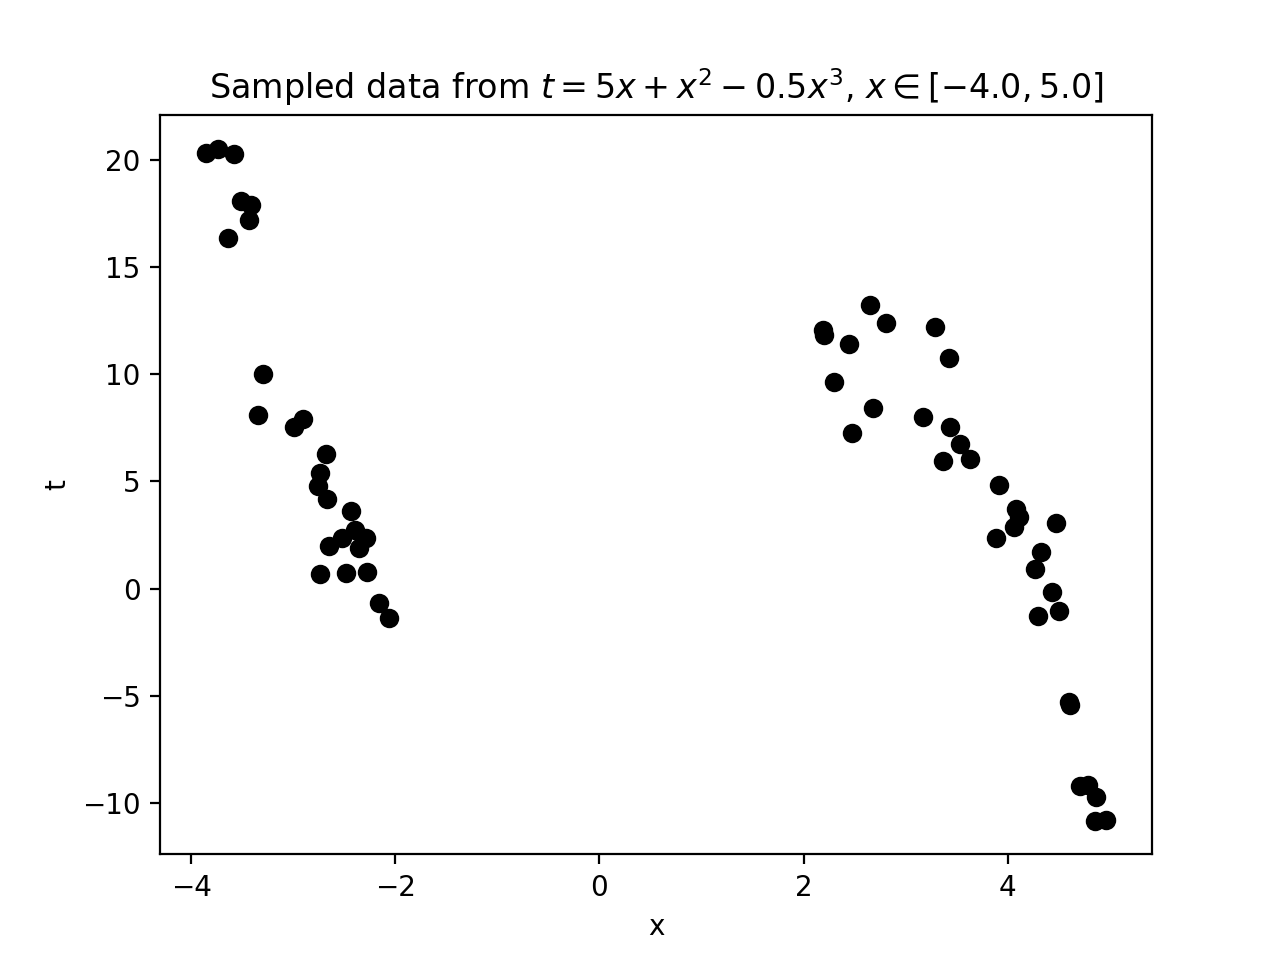
\includegraphics[width=\linewidth]{data.png}
 \caption{This is a sample of the data generated by our true 
 function with a gap introduced by deleting the values between -2 and 2.}
\label{label}
\end{figure}

\begin{figure}[H]
\centering
  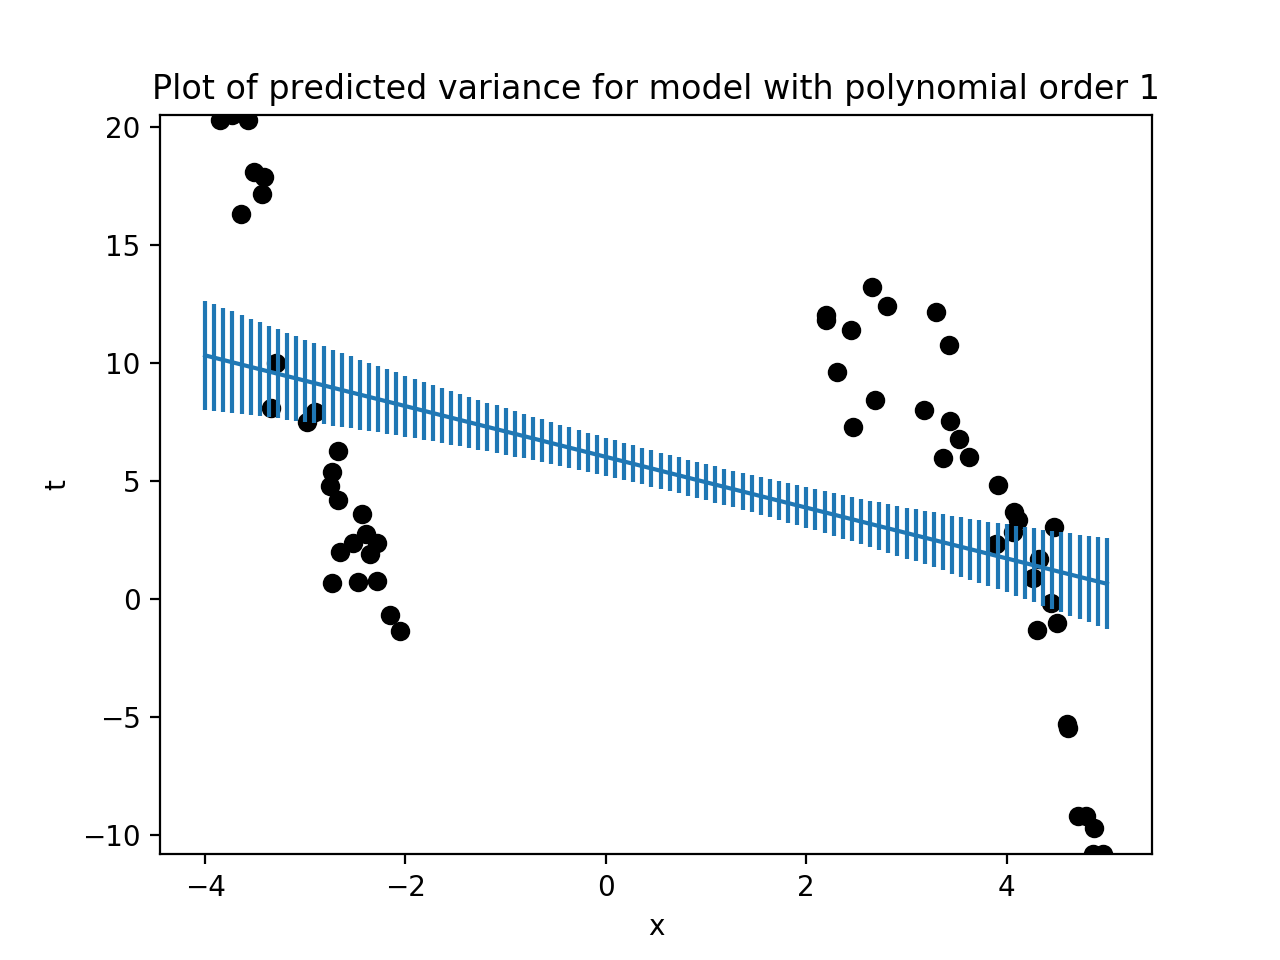
\includegraphics[width=\linewidth]{error-1.png}
 \caption{Predicted error model 1: Limited to a straight line, the 1st order model can do little better than estimate a slope through the means of the two clusters.}
\label{label}
\end{figure}

\begin{figure}[H]
\centering
  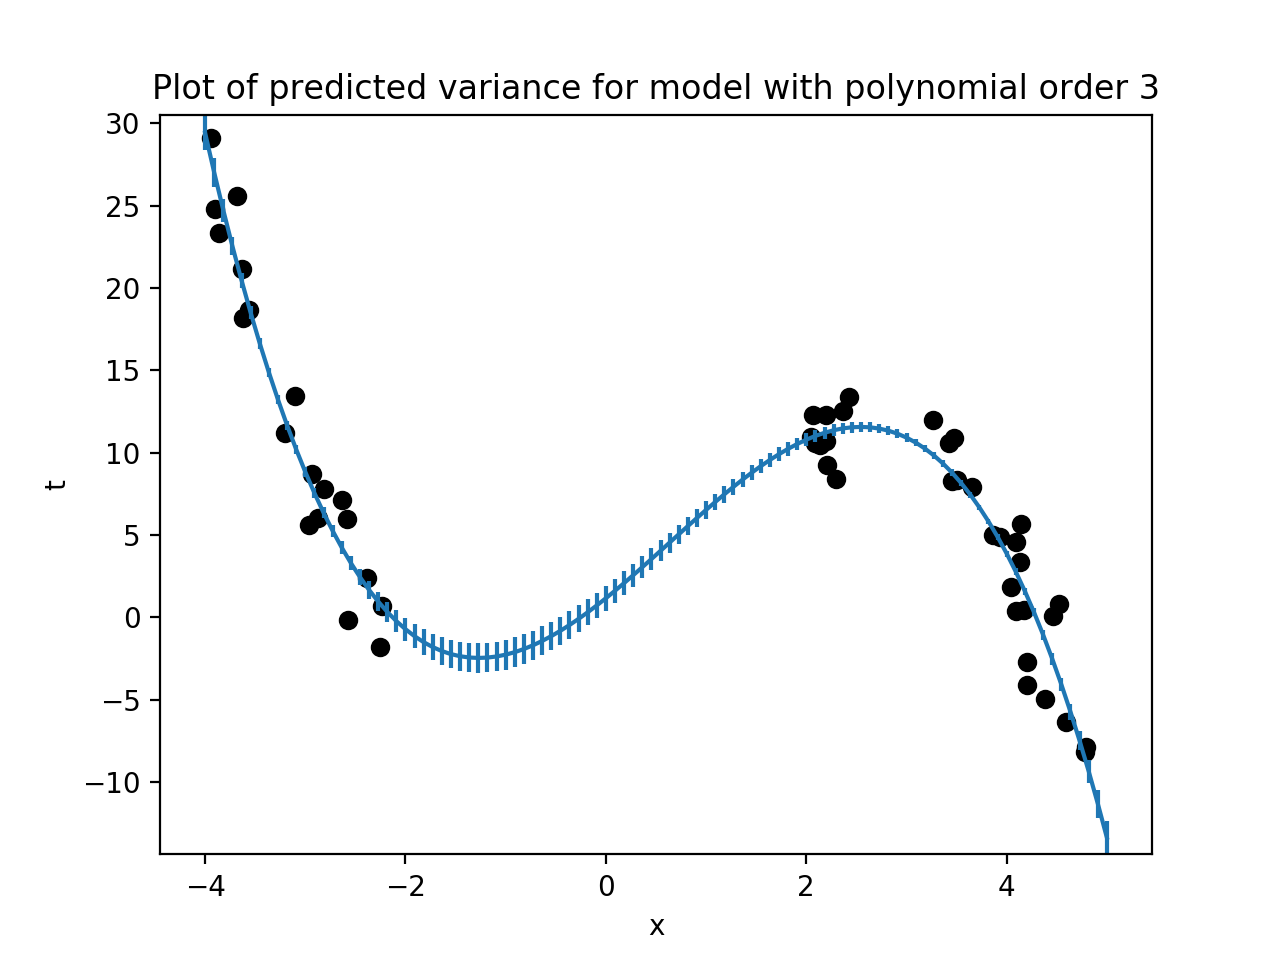
\includegraphics[width=\linewidth]{error-3.png}
 \caption{Predicted error model 3: The third order includes enough parameters to fit a curve that closely resembles the original function. The error bars, however, indicate there is some uncertainty in the gap, but it's not much because we are really close to the true function.}
\label{label}
\end{figure}

\begin{figure}[H]
\centering
  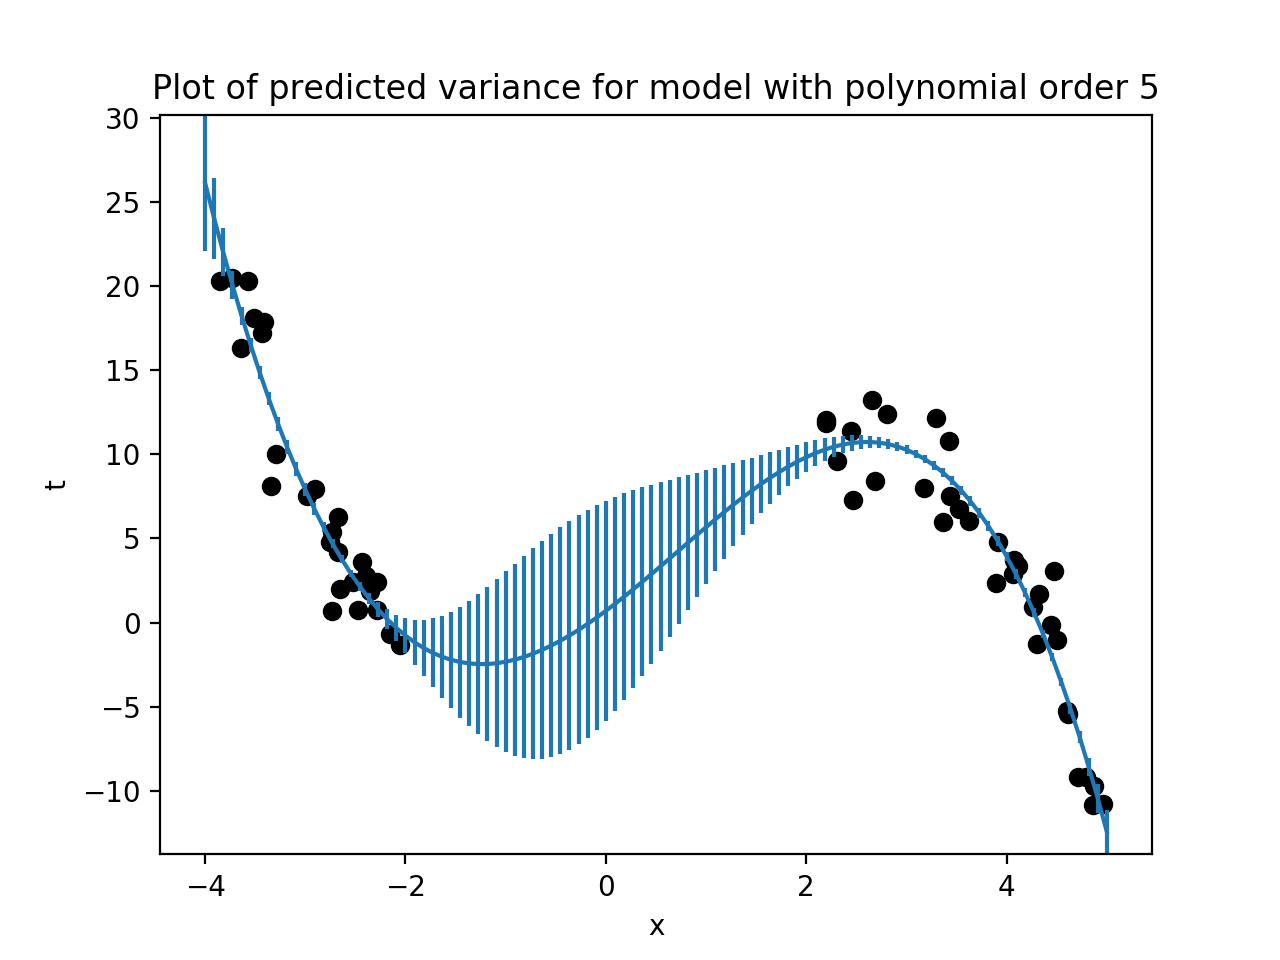
\includegraphics[width=\linewidth]{error-5.png}
 \caption{Predicted error model 5: While the fifth order is more flexible through the provided data points, this model is much more uncertain in the gaps as indicated by the wider error bars.}
\label{label}
\end{figure}

\begin{figure}[H]
\centering
  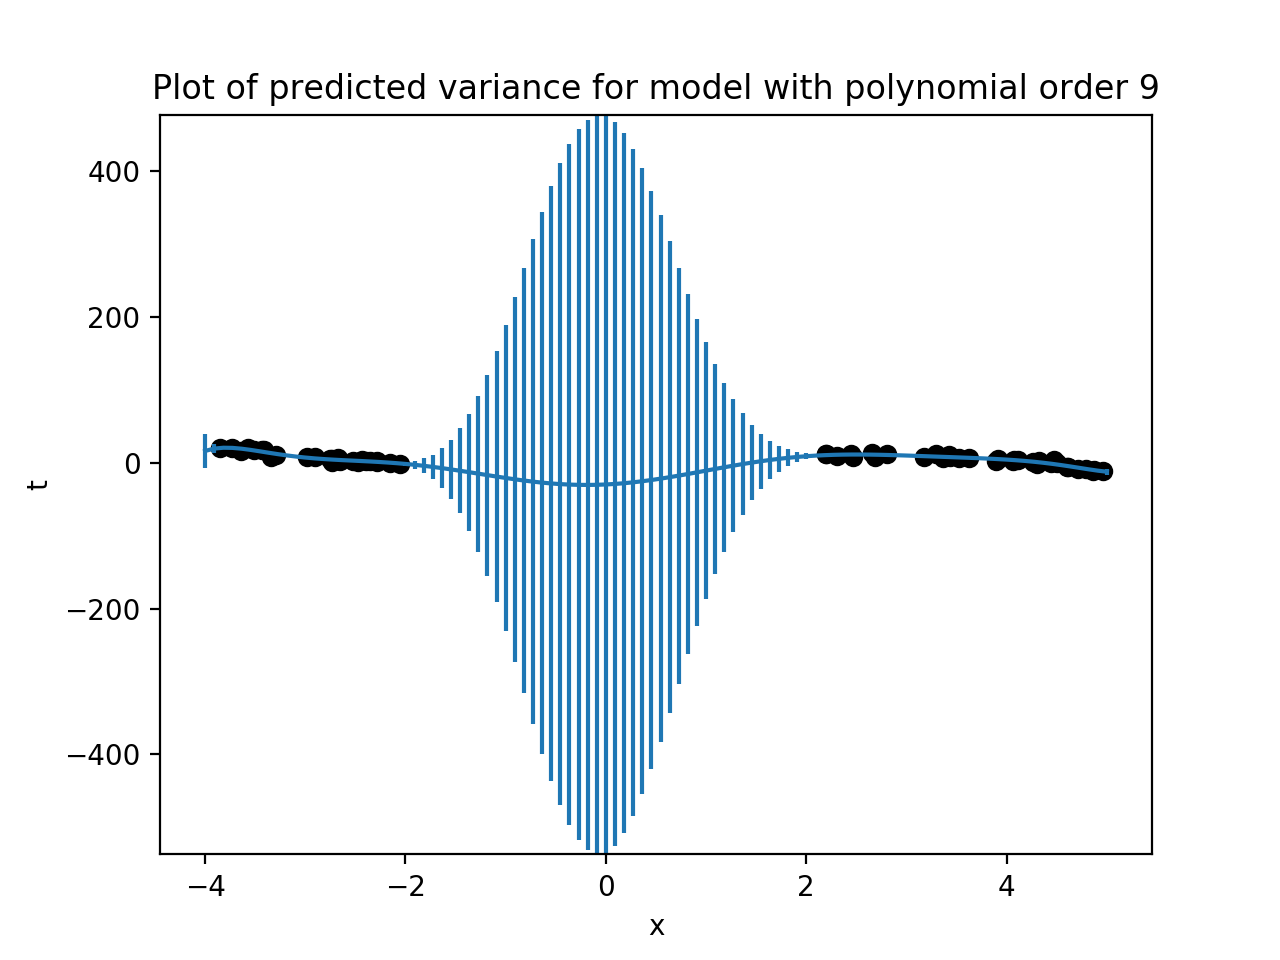
\includegraphics[width=\linewidth]{error-9.png}
 \caption{Predicted error model 9: The ninth order can hit almost every provided data point, but the error explodes in the gap, pushing the curve into almost a line to accommodate the wide error margins.}
\label{label}
\end{figure}

\begin{figure}[H]
\centering
  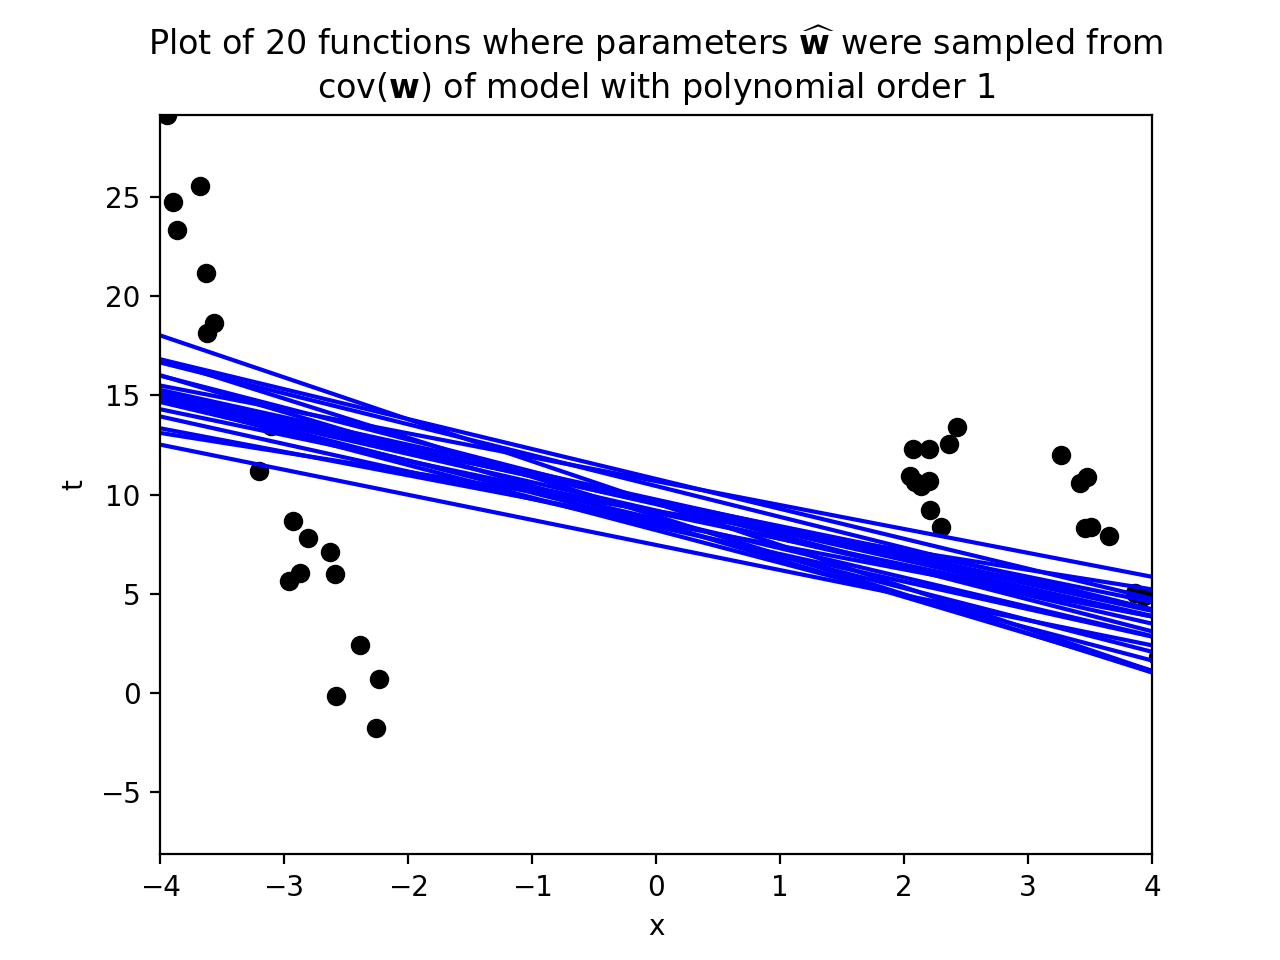
\includegraphics[width=\linewidth]{sampled-fns-1.png}
 \caption{Sampled covariance model 1: The 20 first-order models roughly capture the same slope through the gap, but there is a good deal of variability from line to line.}
\label{label}
\end{figure}

\begin{figure}[H]
\centering
  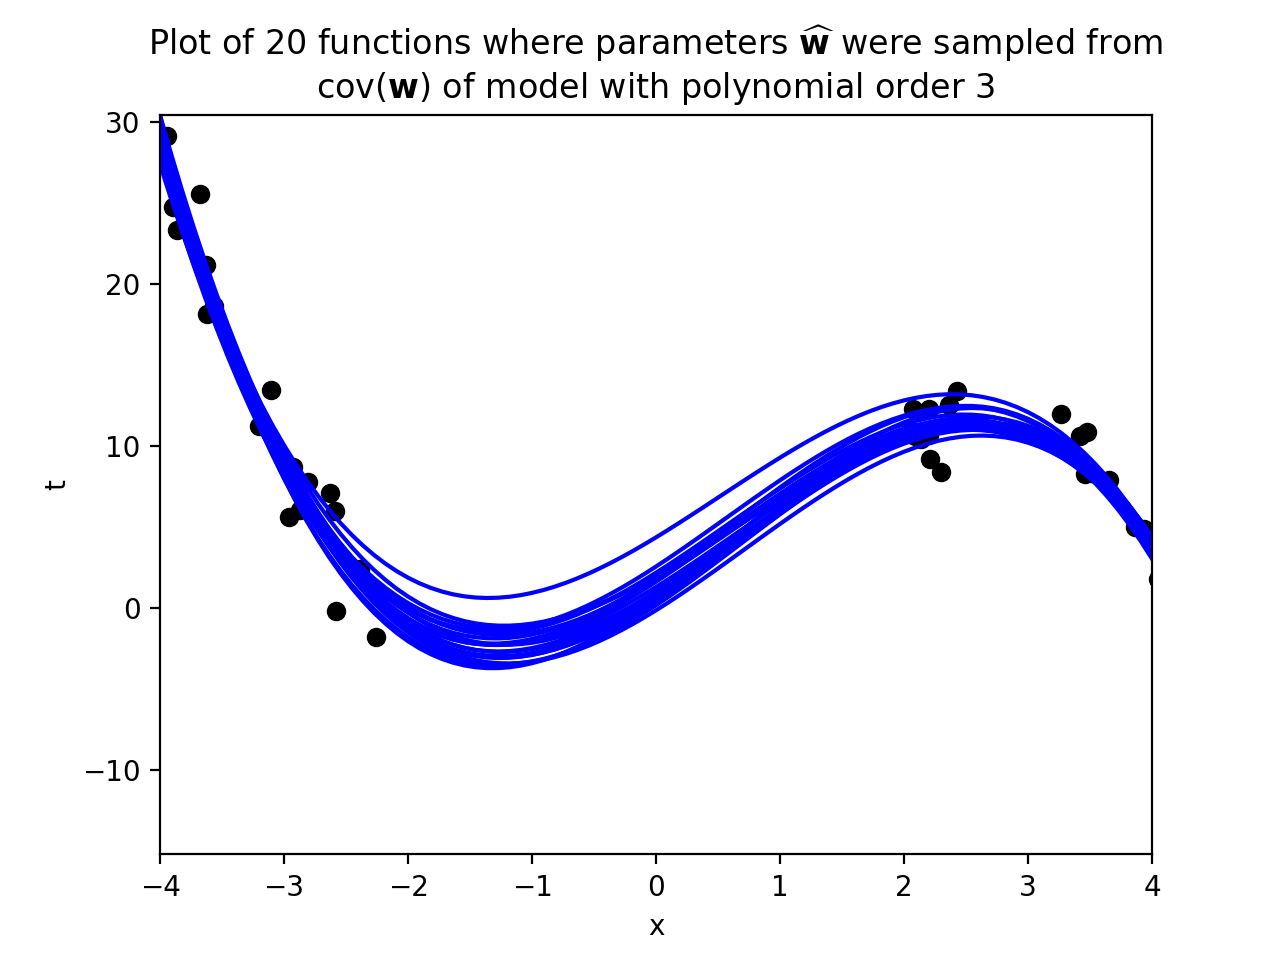
\includegraphics[width=\linewidth]{sampled-fns-3.png}
 \caption{Sampled covariance model 3: The third order, being of the same order as the true function, form almost a single ribbon due to the agreement in the samples.}
\label{label}
\end{figure}

\begin{figure}[H]
\centering
  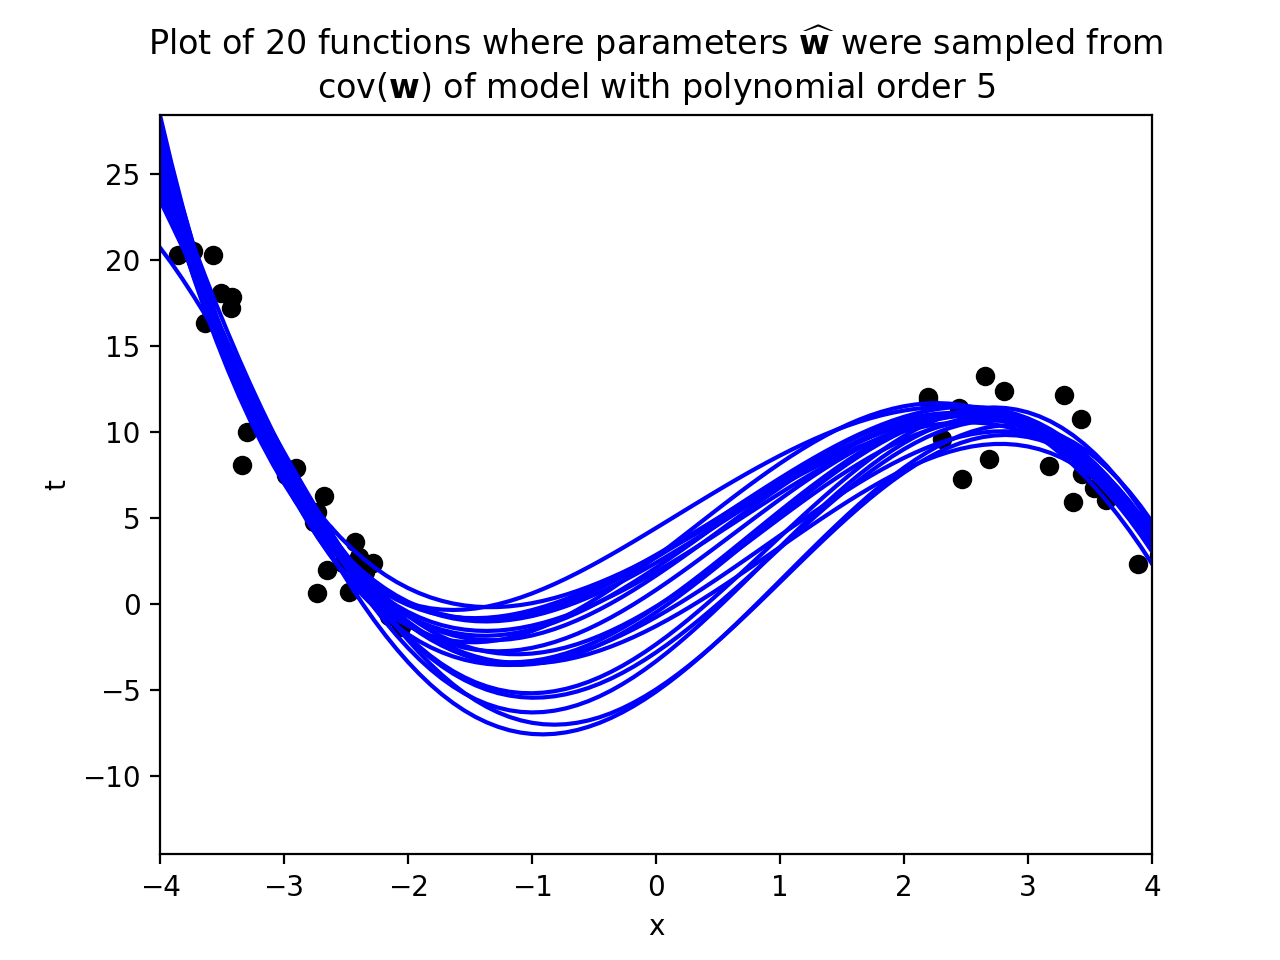
\includegraphics[width=\linewidth]{sampled-fns-5.png}
 \caption{Sampled covariance model 5: The fifth-order curves do well in the places where there is supporting data but begin to vary considerably in how they best estimate how to cross the gap.}
\label{label}
\end{figure}

\begin{figure}[H]
\centering
  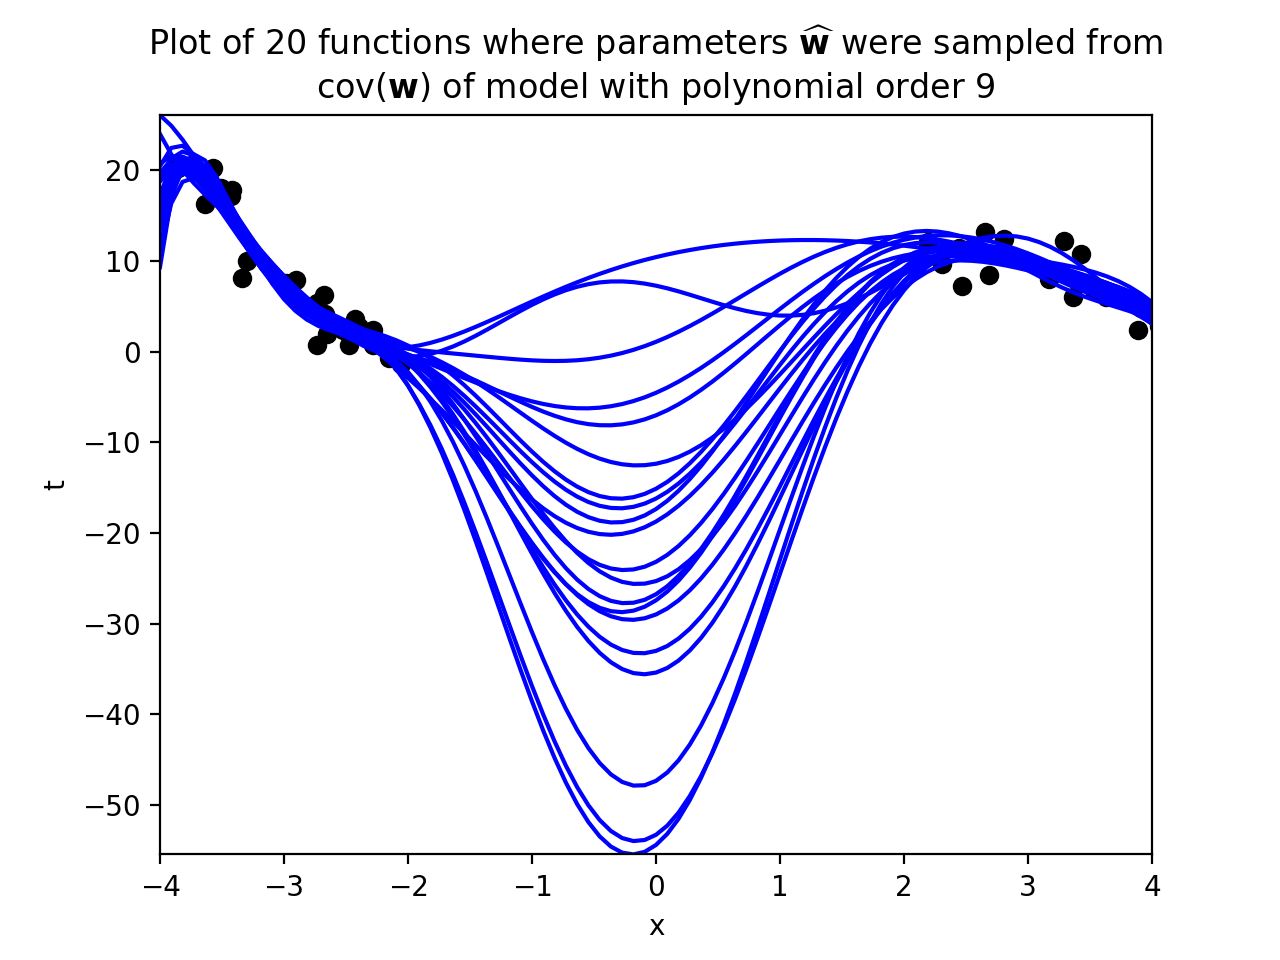
\includegraphics[width=\linewidth]{sampled-fns-9.png}
 \caption{Sampled covariance model 9: The ninth-order model is solid over the provided data but goes fairly wobbly in the gap providing almost unusable data.}
\label{label}
\end{figure}

When the -2/2 data points are not removed, each successive model over 1 looks pretty good and has very little error. 

%%%     Problem 6
\item[6.] [5 points]

In this exercise, you will create a new script that demonstrates how model bias impacts variance, similar to the demonstration in Lecture 9 (starting slide 28).  In your submission, you will name the file for your script {\tt model\_bias\_variance.py}.  You will copy the functions {\tt true\_function} and {\tt sample\_from\_function} from {\tt predictive\_variance.py}.  Using {\tt true\_function} (which computes $t = 5x + x^2 - 0.5x^3$), generate 20 data sets, each consisting of 25 samples from the true function (using the same range of $x \in [-4.0, 5.0]$ and {\tt noise\_var} $= 6$), using the function {\tt sample\_from\_function}.  Then, create a separate plot for each of the model polynomial orders 1, 3, 5 and 9, in which you plot the true function in red and each of the best fit functions (in blue) of that model order to each of the 20 data sets.  You will therefore produce four plots.  The first will be for model order 1 and will include the true model plotted in red and then 20 blue curves, one each for an order 1 best fit model for each of the 20 data set, for all data sets.  The second plot will repeat this for model order 3, and so on.  You can use any of the code in the script {\tt predictive\_variance.py} as a guide.  In your written answer, describe what happens to the variance in the functions in the plots as the model order is changed.  (tips: plot the red true function curve last, so it is plotted on top of the others; also, use {\tt linewidth=3} in the plot fn to increase the line width to make the red true model curve stand out more.)

{\bf Solution.} 

\begin{figure}[H]
\centering
  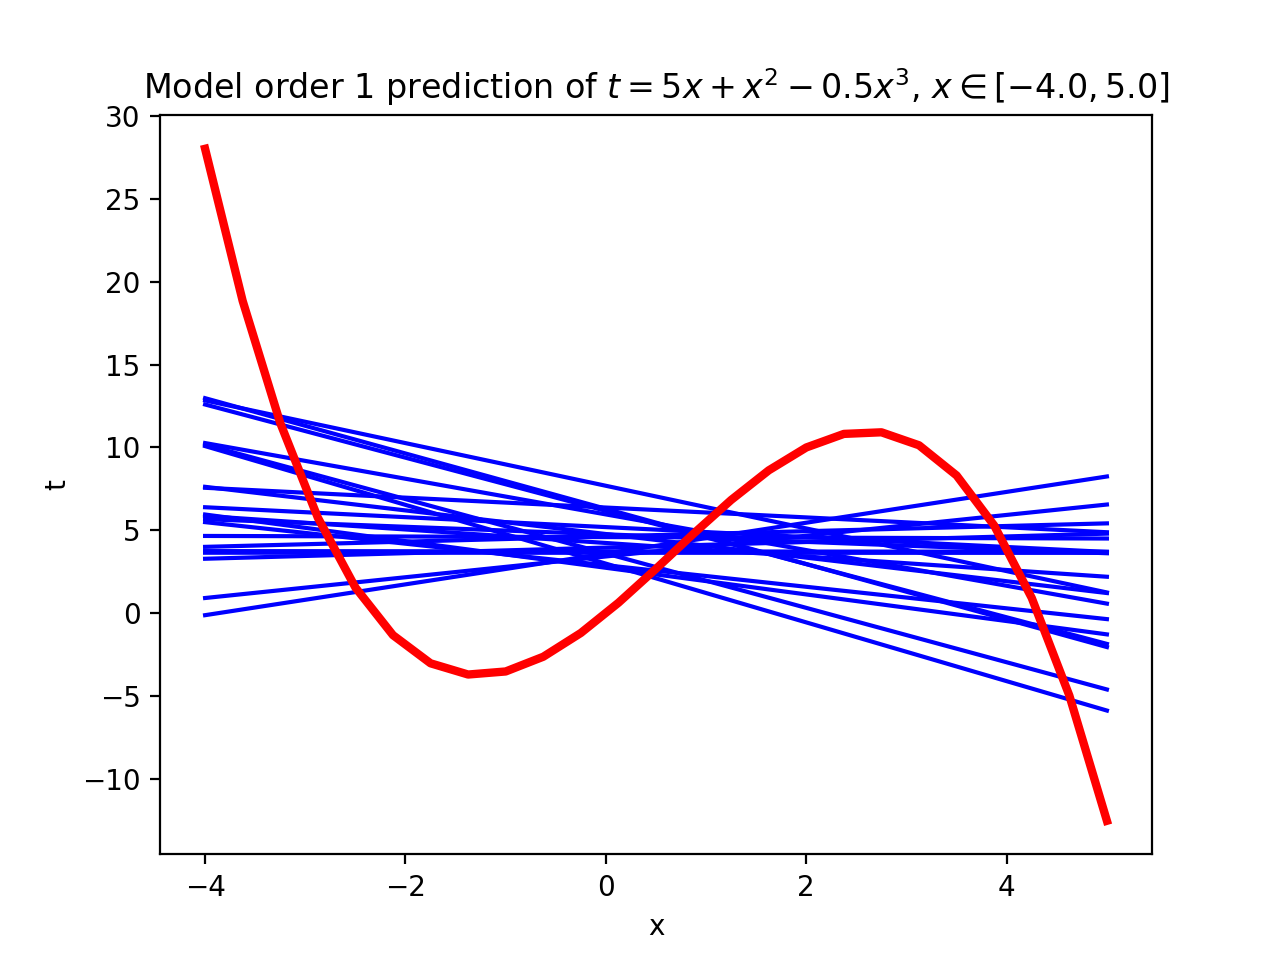
\includegraphics[width=\linewidth]{model_bias-1.png}
 \caption{Prediction of function with model order 1: This model contains too little flexibility and so basically predicts a flat line.}
\label{label}
\end{figure}

\begin{figure}[H]
\centering
  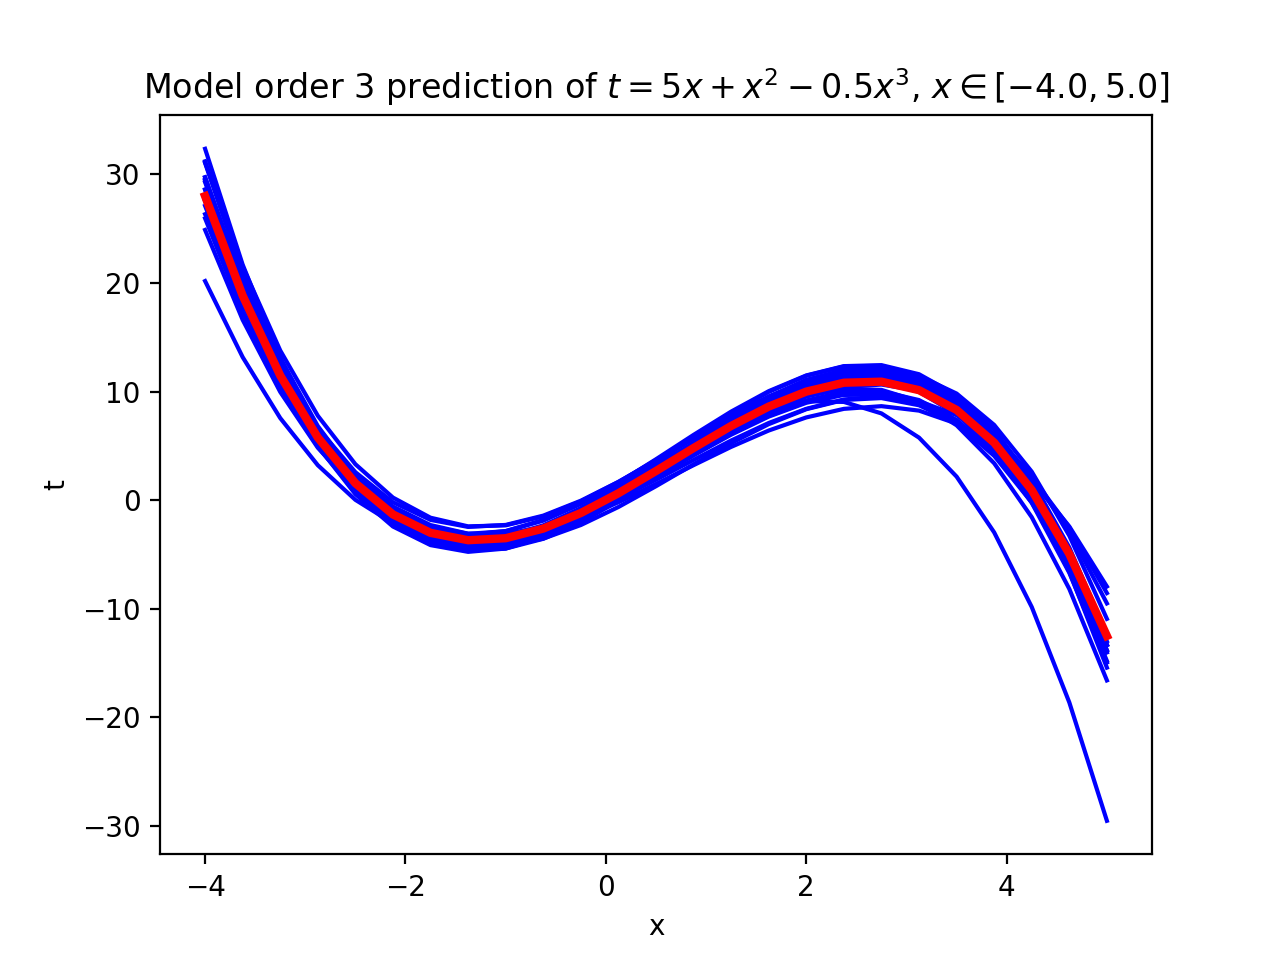
\includegraphics[width=\linewidth]{model_bias-3.png}
 \caption{Prediction of function with model order 3: This model is of the same order as the true function and so the lines are almost indistinguishable from each other.}
\label{label}
\end{figure}

\begin{figure}[H]
\centering
  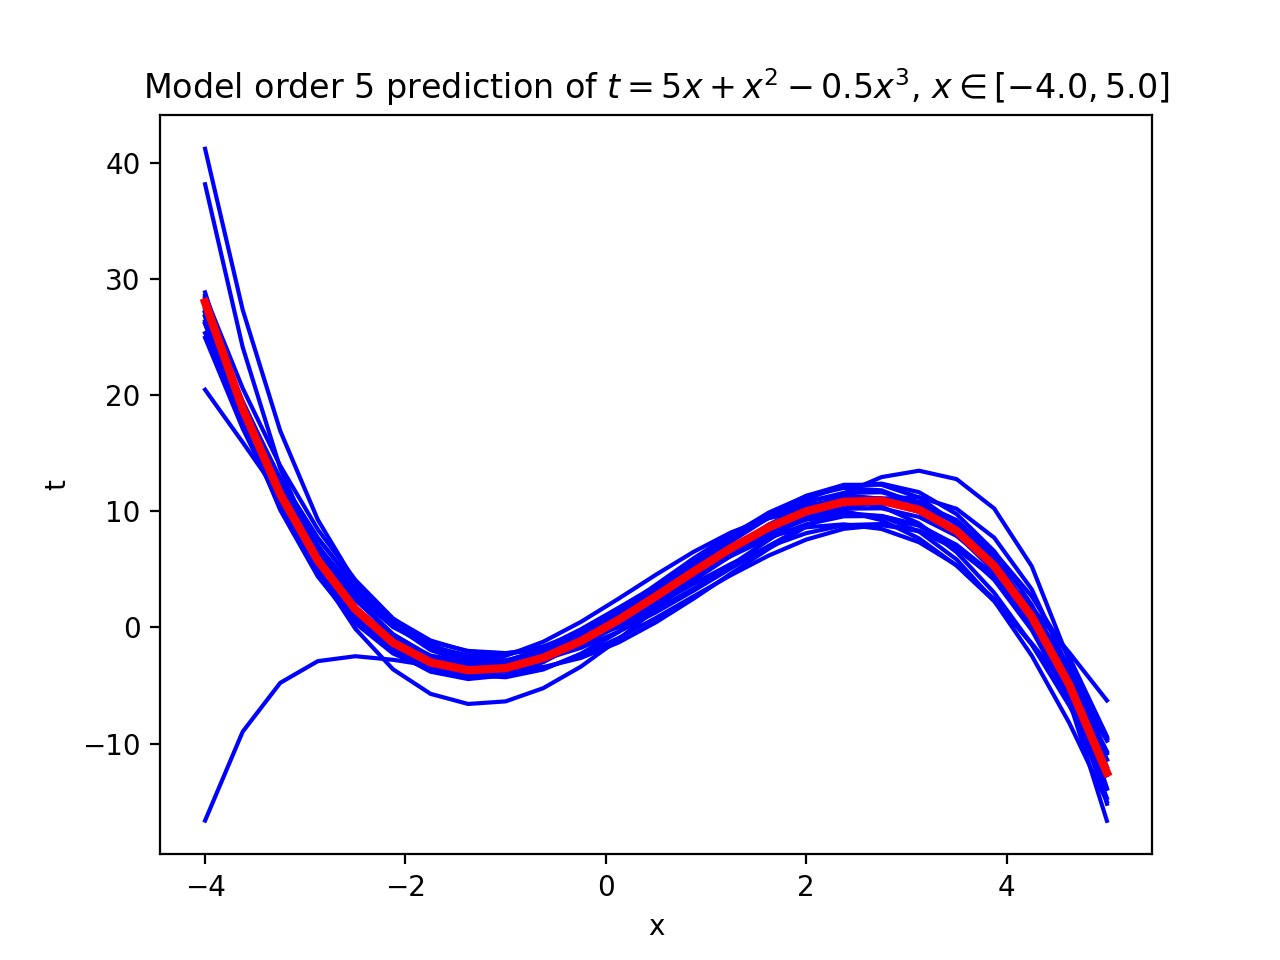
\includegraphics[width=\linewidth]{model_bias-5.png}
 \caption{Prediction of function with model order 5: The bias introduced by this more flexible model is shown by how the blue lines are more spread out from each other.}
\label{label}
\end{figure}

\begin{figure}[H]
\centering
  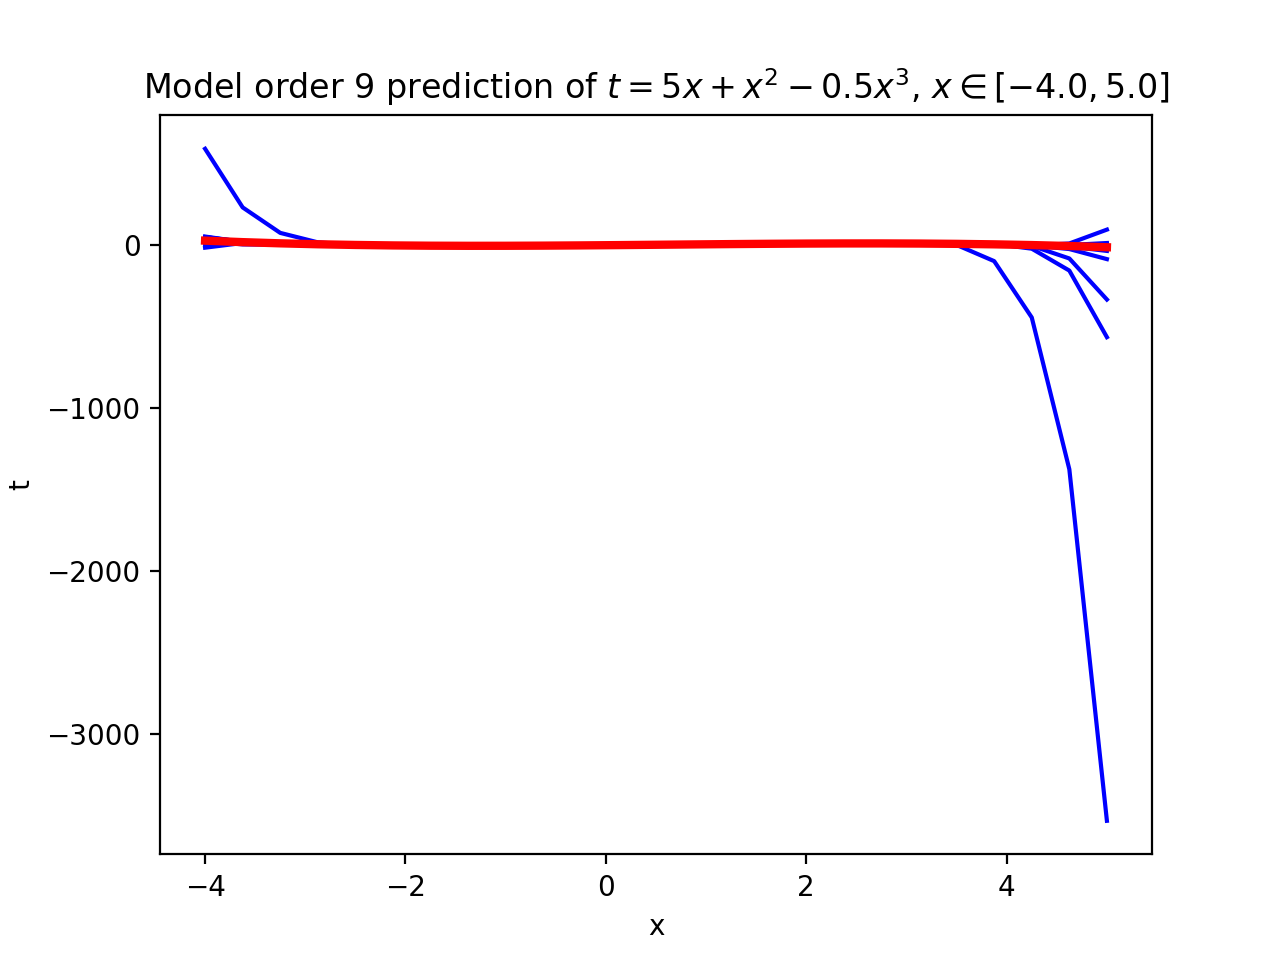
\includegraphics[width=\linewidth]{model_bias-9.png}
 \caption{Prediction of function with model order 9: From run to run, this model looks wildly different because of the extremity of the model's order. }
\label{label}
\end{figure}

The variance increases with model order, introducing greater variability in the predictions.

%%%     Problem 7
\item[7.] [3 points; \boldred{Required only for Graduates}]
Adapted from {\bf Exercise 2.13} of FCML:

Compute the Fisher Information Matrix for the parameter of a Bernoulli distribution.

{\bf Solution.}

\begin{eqnarray*}
\begin{aligned}
P(x|q) &= q^x(1-q)^{1-x}
\\
\mathcal{L} &= \prod_n^N q^{x_n}(1-q)^{1-{x_n}}
\\
\log\mathcal{L} &= \sum_n^N \log \left( q^{x_n} (1-q)^{1-{x_n}} \right)
\\
\frac { \partial \log\mathcal{L}} {\partial q} &= \frac{\sum_n^N x_n}{q} + \frac{\sum_n^N 1 - x_n}{1 - q}
= q^{-1} \sum_n^N x_n + (1 - q)^{-1} \sum_n^N 1 - x_n
\\
\frac { \partial^2 \log\mathcal{L}} {\partial q} &= - q^{-2} \sum_n^N x_n - (1 - q)^{-2} \sum_n^N 1 - x_n
\\
\mathcal{I} &= \mathrm{E}_{P(x|q)} \{ - \frac { \partial^2 \log\mathcal{L}} {\partial q} \}
\\
\mathrm{E}_{P(x)} \{ f(X) \} &= \sum_x f(x) P(x)
\\
\mathcal{I} &= \sum_x - \frac { \partial^2 \log\mathcal{L}} {\partial q} P(x|q)
\\
P(x|q) &= (1 * q) + (0 * (1 - q)) = q
\\
\mathcal{I} &= \sum_x - \frac { \partial^2 \log\mathcal{L}} {\partial q} q
\\
&= -q \sum_x \frac { \partial^2 \log\mathcal{L}} {\partial q}
\end{aligned}
\end{eqnarray*}

I think this is probably the answer. I hope I've sufficiently proven $P(x|q) = q$. I confess I do not understand how this is a matrix. Won't this be a scalar value in the end?

I had done some additional distribution of terms which I'm not sure is necessary:

\begin{eqnarray*}
\begin{aligned}
\mathcal{I} &= \sum_{x=n}^N \left[ - \left(- q^{-2} \sum_n^N x_n - (1 - q)^{-2} \sum_n^N 1 - x_n \right) q \right]
\\
&= \sum_{x=n}^N \left[ q \left( \frac{\sum_n^N x_n}{q^2} + \frac{\sum_n^N 1 - x_n}{(1 - q)^{2}} \right) \right]
\\
&= \sum_{x=n}^N \left[ q \left( \frac{\sum_n^N x_n}{q^2} + \frac{N - \sum_n^N x_n}{(1 - q)^{2}} \right) \right]
\\
&= \sum_{x=n}^N \left[ \frac{q \sum_n^N x_n}{q^2} + \frac{qN - q \sum_n^N x_n}{(1 - q)^{2}} \right]
\\
&= \sum_{x=n}^N \left[ \frac{\sum_n^N x_n}{q} + \frac{qN - q \sum_n^N x_n}{(1 - q)^{2}} \right]
\end{aligned}
\end{eqnarray*}

I have no idea how to handle the outer summation over the inner summation or if I should be worried about using different subscripts. 
\end{itemize}

\end{document}